\section{Evaluation}
\label{sec:evaluation}

We evaluate \textsc{G-port} as a runtime scheduling layer, not a new code
construction.  The evaluation first compares \textsc{G-port} with same-runtime
external adapters across TCP, stressed TCP, and K3s worker services, then
isolates design choices, guard sensitivity, stress recovery, and row-exposure
mechanisms.  The main comparison reports latency, tail latency, throughput, work
overhead, cancellation cost, and decode success; later diagnostics reuse the
decision and recovery counters from Section~\ref{sec:setup}.

\subsection{Main External Comparison}

Table~\ref{tab:external-main} is the main systems result.  Every row uses the
same payloads, worker-state streams, cancellation path, and barrier accounting
inside that runtime.  RLTune and Sailor are same-runtime scheduler adapters, not
full system ports; they test whether generic heterogeneity-aware scheduling is
enough once the runtime and workload are held fixed.  The table reports raw
metrics rather than normalized gains: mean barrier latency, p95 barrier latency,
achieved iteration throughput, post-decode rows, cancellation time, and decode
success.

\begin{table*}[t]
  \centering
  \caption{Main external comparison.}
  \label{tab:external-main}
  \begin{tabular*}{\textwidth}{@{\extracolsep{\fill}}lllrrrrrr@{}}
    \toprule
    Runtime & Workers & Method & Mean & p95 & Thr. & Post & Cancel & Succ. \\
            &         &        & (ms) & (ms) & (iter/s) & rows & (ms) & \\
    \midrule
    TCP & W8 & SFCL & 44.0 & 80.5 & 22.7 & 1.8 & 16.8 & 1.00 \\
        &    & RLTune & 48.2 & 76.6 & 20.8 & 0.1 & 16.5 & 1.00 \\
        &    & Sailor & 53.9 & 77.8 & 18.6 & 0.0 & 19.2 & 1.00 \\
        &    & \textsc{G-port} & \textbf{40.9} & \textbf{71.5} & \textbf{24.4} & 1.6 & 14.1 & 1.00 \\
        & W16 & SFCL & 38.3 & \textbf{48.3} & 26.1 & 10.4 & 16.5 & 1.00 \\
        &     & RLTune & 36.4 & 59.1 & 27.4 & 1.4 & 16.5 & 1.00 \\
        &     & Sailor & \textbf{35.3} & 59.5 & \textbf{28.3} & 0.0 & 16.3 & 1.00 \\
        &     & \textsc{G-port} & 36.6 & 60.0 & 27.4 & 4.1 & 16.9 & 1.00 \\
        & W24 & SFCL & 47.5 & 62.3 & 21.1 & 21.9 & 21.4 & 1.00 \\
        &     & RLTune & 48.3 & \textbf{59.9} & 20.7 & 2.8 & 24.2 & 1.00 \\
        &     & Sailor & 44.3 & 61.1 & 22.6 & 0.0 & 21.8 & 1.00 \\
        &     & \textsc{G-port} & \textbf{43.7} & 61.1 & \textbf{22.9} & 1.7 & 20.5 & 1.00 \\
    \midrule
    TCP+stress & W8 & SFCL & 49.4 & 88.6 & 20.2 & 1.4 & 15.2 & 1.00 \\
        &    & RLTune & 55.6 & 86.0 & 18.0 & 0.3 & 17.1 & 1.00 \\
        &    & Sailor & 56.3 & 89.9 & 17.8 & 0.0 & 15.8 & 1.00 \\
        &    & \textsc{G-port} & \textbf{48.4} & \textbf{73.9} & \textbf{20.7} & 1.6 & 15.2 & 1.00 \\
        & W16 & SFCL & 53.2 & \textbf{71.0} & 18.8 & 9.8 & 23.6 & 1.00 \\
        &     & RLTune & 53.1 & 77.0 & 18.8 & 1.5 & 22.5 & 1.00 \\
        &     & Sailor & 53.3 & 71.2 & 18.7 & 0.0 & 22.2 & 1.00 \\
        &     & \textsc{G-port} & \textbf{53.1} & 83.9 & \textbf{18.8} & 0.0 & 22.2 & 1.00 \\
        & W24 & SFCL & 60.9 & 93.3 & 16.4 & 21.0 & 27.2 & 1.00 \\
        &     & RLTune & 65.4 & 137.5 & 15.3 & 4.1 & 29.8 & 1.00 \\
        &     & Sailor & 55.5 & 67.6 & 18.0 & 0.0 & 23.9 & 1.00 \\
        &     & \textsc{G-port} & \textbf{53.9} & \textbf{61.2} & \textbf{18.5} & 0.0 & 23.7 & 1.00 \\
    \midrule
    K3s & W8 & SFCL & 22.7 & 60.3 & 44.0 & 0.4 & 1.7 & 1.00 \\
        &    & RLTune & 28.0 & 55.5 & 35.7 & 0.0 & 1.6 & 1.00 \\
        &    & Sailor & 29.0 & 54.4 & 34.5 & 0.0 & 1.6 & 1.00 \\
        &    & \textsc{G-port} & \textbf{19.6} & \textbf{42.0} & \textbf{51.0} & 0.4 & 1.7 & 1.00 \\
        & W16 & SFCL & 14.5 & 16.3 & 69.1 & 3.4 & 3.6 & 1.00 \\
        &     & RLTune & 9.8 & 10.9 & 102.0 & 1.3 & 3.2 & 1.00 \\
        &     & Sailor & \textbf{9.4} & \textbf{10.2} & \textbf{106.7} & 0.0 & 2.9 & 1.00 \\
        &     & \textsc{G-port} & 11.3 & 16.0 & 88.3 & 1.5 & 3.2 & 1.00 \\
        & W24 & SFCL & 15.7 & 17.6 & 63.6 & 8.9 & 5.6 & 1.00 \\
        &     & RLTune & 12.8 & 14.8 & 78.2 & 2.5 & 4.6 & 1.00 \\
        &     & Sailor & \textbf{12.4} & 13.3 & \textbf{80.8} & 0.0 & 4.3 & 1.00 \\
        &     & \textsc{G-port} & 12.4 & \textbf{13.2} & 80.5 & 0.0 & 4.3 & 1.00 \\
    \bottomrule
  \end{tabular*}
\end{table*}

The table makes the runtime boundary explicit: the same adapter set runs under
local TCP, stressed TCP, and pod-to-pod K3s services.  Generic heterogeneity
schedulers improve selected W16/W24 cases but regress at W8 because they do not
control which coded rows make the first decodable prefix appear.  \textsc{G-port}
is not always fastest (Sailor wins some K3s W16/W24 speed-dominated cases), but
it has the best W8 mean/p95 in all three runtimes, the best stressed-TCP W24
mean/p95, and competitive K3s W24 throughput.  The integrated overhead rows show
that the gain is not only a latency artifact: \textsc{G-port} usually leaves
fewer post-decode rows than SFCL and preserves decode success while cancellation
time remains included in the barrier path.  The artifact keeps completed rows,
extra work, dispatch time, bytes, per-seed traces, paired gains, and paired CIs.

\subsection{Ablation Study}

Table~\ref{tab:gport-ablation} removes deployable pieces of \textsc{G-port} in
all three runtimes.  \emph{w/o FD} removes first-decode-aware row ordering and
therefore becomes the Sailor-style speed/cost scheduler.  \emph{w/o code}
removes the code-aware candidate and becomes the RLTune-style heterogeneity
selector.  \emph{w/o portfolio} disables the cross-policy wrapper and runs the
coded-only \textsc{Guard-D} arm.  Each cell is mean latency / post-decode rows /
cancellation time; lower is better.

\begin{table*}[t]
  \centering
  \caption{\textsc{G-port} ablations.}
  \label{tab:gport-ablation}
  \begin{tabular*}{\textwidth}{@{\extracolsep{\fill}}llccc@{}}
    \toprule
    Runtime & Ablation & W8 & W16 & W24 \\
    \midrule
    \multicolumn{5}{@{}l@{}}{\emph{Cell:} mean ms / post rows / cancel ms} \\
    \midrule
    TCP & \textsc{G-port} & 40.9/1.6/14.1 & 36.6/4.1/16.9 & 43.7/1.7/20.5 \\
        & w/o FD          & 53.9/0.0/19.2 & 35.3/0.0/16.3 & 44.3/0.0/21.8 \\
        & w/o code        & 48.2/0.1/16.5 & 36.4/1.4/16.5 & 48.3/2.8/24.2 \\
        & w/o portfolio   & 43.3/1.6/17.6 & 38.5/10.6/15.4 & 47.0/22.1/21.0 \\
    \midrule
    TCP+stress & \textsc{G-port} & 48.4/1.6/15.2 & 53.1/0.0/22.2 & 53.9/0.0/23.7 \\
        & w/o FD          & 56.3/0.0/15.8 & 53.3/0.0/22.2 & 55.5/0.0/23.9 \\
        & w/o code        & 55.6/0.3/17.1 & 53.1/1.5/22.5 & 65.4/4.1/29.8 \\
        & w/o portfolio   & 47.9/2.0/15.3 & 55.8/11.1/24.8 & 54.7/19.7/24.6 \\
    \midrule
    K3s & \textsc{G-port} & 19.6/0.4/1.7 & 11.3/1.5/3.2 & 12.4/0.0/4.3 \\
        & w/o FD          & 29.0/0.0/1.6 & 9.4/0.0/2.9 & 12.4/0.0/4.3 \\
        & w/o code        & 28.0/0.0/1.6 & 9.8/1.3/3.2 & 12.8/2.5/4.6 \\
        & w/o portfolio   & 20.3/0.5/1.7 & 14.2/3.6/3.6 & 15.9/9.1/5.7 \\
    \bottomrule
  \end{tabular*}
\end{table*}

The ablation shows why the full controller is useful.  Speed/cost scheduling is
strong when speed dominates (K3s W16/W24) but fragile at W8 and under TCP stress.
The heterogeneity selector helps selected counts but has the largest stressed-TCP
W24 latency.  The w/o-portfolio variant is a clean coded-only ablation and
competitive at W8, but it loses the cross-policy fallback that protects
\textsc{G-port} when uncoded or speed-aware execution is temporarily safer.

\subsection{Guard Sensitivity}

\begin{figure}[t]
  \centering
  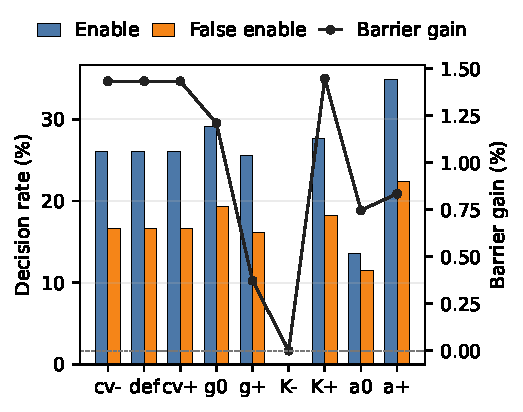
\includegraphics[width=\columnwidth]{figures/guard_threshold_sensitivity.pdf}
  \caption{Guard-threshold sensitivity.}
  \Description{Bar and line chart showing enable rate, false-enable rate, and
  barrier gain under small guard-threshold changes.}
  \label{fig:guard-thresholds}
\end{figure}

\begin{table}[t]
  \centering
  \caption{Figure~\ref{fig:guard-thresholds} settings.}
  \label{tab:guard-threshold-settings}
  \begin{tabular}{@{}lrrrr@{}}
    \toprule
    Label & theta-cv & theta-g & theta-K & theta-a \\
    \midrule
    low theta-cv & 0.10 & 0.01 & 0 & 1 \\
    default & 0.20 & 0.01 & 0 & 1 \\
    high theta-cv & 0.35 & 0.01 & 0 & 1 \\
    zero theta-g & 0.20 & 0.00 & 0 & 1 \\
    high theta-g & 0.20 & 0.03 & 0 & 1 \\
    strict theta-K & 0.20 & 0.01 & -1 & 1 \\
    loose theta-K & 0.20 & 0.01 & 1 & 1 \\
    strict theta-a & 0.20 & 0.01 & 0 & 0 \\
    loose theta-a & 0.20 & 0.01 & 0 & 2 \\
    \bottomrule
  \end{tabular}
\end{table}

Figure~\ref{fig:guard-thresholds} replays small threshold changes on paired K3s
guard rounds, and Table~\ref{tab:guard-threshold-settings} maps each x-axis
label to the guard rule.  Each non-default setting changes one gate while
holding the other three at the deployed default.  Here
theta-cv gates worker-speed heterogeneity, theta-g gates
predicted first-decode gain, theta-K gates the candidate-minus-fallback
first-decodable prefix delta, and theta-a gates rows of work completed after
decode.  Lower theta-K or theta-a values are stricter because they allow
less prefix growth or post-decode work.  Bars report enable decision rate and
false-enable rate; the line shows barrier gain.  Stricter thresholds reduce
false enables but also leave useful opportunities unused, so the default is a
conservative middle point rather than a tuned post-hoc optimum.

\subsection{Stress and Recovery}

Table~\ref{tab:k8s-stress} reports K3s W24 stress tests using the correctness
and recovery counters from Section~\ref{sec:setup}.  \emph{Stress} is the
injected runtime condition, not a new workload: Base has no injection, Cancel+20
delays cancellation, CPU hog adds co-located interference, Close closes one
worker connection, and Close+R repeats Close with bounded reissue.  Succ. is
decode success; Gain is relative to SFCL in the same stress; Err. and Recov. are
closed-worker errors and bounded reissues per round.

\begin{table}[t]
  \centering
  \setlength{\tabcolsep}{1.0pt}
  \caption{K3s W24 recovery counters.}
  \label{tab:k8s-stress}
  \begin{tabular}{@{}llrrrrrr@{}}
    \toprule
    Stress & Method & Succ. & Barrier & Gain & Err. & Recov. & Cancel \\
         &        &       & (ms) &      & /round & /round & (ms) \\
    \midrule
    Base & SFCL & 1.00 & 16.6 & 0.0\% & 0.00 & 0.00 & 5.7 \\
    Base & \textsc{G-port} & 1.00 & 12.6 & 23.7\% & 0.00 & 0.00 & 4.4 \\
    Base & Guard-D & 1.00 & 16.6 & -0.3\% & 0.00 & 0.00 & 5.6 \\
    \midrule
    Cancel+20 & SFCL & 1.00 & 33.7 & 0.0\% & 0.00 & 0.00 & 24.8 \\
    Cancel+20 & \textsc{G-port} & 1.00 & 32.0 & 5.1\% & 0.00 & 0.00 & 23.6 \\
    Cancel+20 & Guard-D & 1.00 & 33.9 & -0.7\% & 0.00 & 0.00 & 24.7 \\
    \midrule
    CPU hog & SFCL & 1.00 & 16.6 & 0.0\% & 0.00 & 0.00 & 5.6 \\
    CPU hog & \textsc{G-port} & 1.00 & 12.5 & 24.8\% & 0.00 & 0.00 & 4.3 \\
    CPU hog & Guard-D & 1.00 & 16.5 & 0.6\% & 0.00 & 0.00 & 5.5 \\
    \midrule
    Close & SFCL & 1.00 & 16.7 & 0.0\% & 1.00 & 0.00 & 5.5 \\
    Close & \textsc{G-port} & 0.67 & 10.8 & 35.0\% & 1.00 & 0.00 & 2.8 \\
    Close & Guard-D & 1.00 & 16.6 & 0.1\% & 1.00 & 0.00 & 5.5 \\
    \midrule
    Close+R & SFCL & 1.00 & 16.8 & 0.0\% & 1.00 & 1.00 & 5.7 \\
    Close+R & \textsc{G-port} & 1.00 & 12.7 & 24.2\% & 1.00 & 0.33 & 4.4 \\
    Close+R & Guard-D & 1.00 & 16.8 & 0.2\% & 1.00 & 1.00 & 5.7 \\
    \bottomrule
  \end{tabular}
\end{table}

The cases separate cleanup, interference, and connection-loss effects.  CPU hog
keeps the gain, while delayed cancellation shrinks it to 5.1\%.  Close without
recovery is only a diagnostic failure mode: fast successful rounds but 67\%
decode success.  Bounded reissue restores success to 1.0 and keeps a 24.2\%
gain, so we claim single-connection recovery semantics rather than production
fault tolerance.

\subsection{Mechanism: Row Exposure}

Table~\ref{tab:score-diagnostic} is an offline 8-worker/8-shard replay, not a
TCP or K3s deployment.  It fixes the code and worker states, changes only
row-pair priority, and measures predicted first-decode time.  The oracle is not
deployable; it only shows the headroom from exposing decode-important rows
earlier.  The cheap runtime score helps p95 but not mean latency, so
\textsc{G-port} treats row score as a guarded runtime feature.

\begin{table}[t]
  \centering
  \setlength{\tabcolsep}{1.0pt}
  \caption{Offline row-exposure replay.}
  \label{tab:score-diagnostic}
  \begin{tabular}{@{}lrrrrr@{}}
    \toprule
    Priority & FD mean & FD p95 & Mean gain & p95 gain & $\Delta$ prefix \\
             & (ms) & (ms) & & & \\
    \midrule
    Static & 31.6 & 117.0 & 0.0\% & 0.0\% & 0.0 \\
    Cost-only & 25.4 & 60.8 & 19.5\% & 48.1\% & -0.4 \\
    Runtime score & 32.8 & 85.6 & -3.8\% & 26.8\% & 0.0 \\
    Oracle-minset & 19.3 & 52.6 & 38.9\% & 55.1\% & -1.2 \\
    Random & 38.2 & 141.2 & -21.1\% & -20.7\% & +0.5 \\
    \bottomrule
  \end{tabular}
\end{table}

Full row-score sweeps, sampled-minset variants, score-build times, and per-seed
ranges are artifact material.  Among the five priorities, \textsc{G-port} uses
the deployable \emph{Runtime score} priority inside its Guard-D coded arm; Static,
Cost-only, Oracle-minset, and Random are controls that respectively represent
the SFCL baseline, a cost-only scheduler, a nondeployable upper-bound oracle, and
a sanity lower bound.  This diagnostic supports a narrow claim: decodability
features create useful candidates, and the online guard decides when to trust the
runtime score.

\subsection{Limitations}

This is a prototype validation: multi-process runs measure sparse kernels; TCP
adds serialization and cancellation; network stress adds analytic RTT/bandwidth;
Docker and K3s validate containerized worker-service paths at local and small
multi-node scales.  The K3s pods do not reserve exclusive CPU or memory.  The
artifact keeps pod placement, events, resource-counter snapshots when available,
and Docker stress hooks for slow cancellation, closed TCP connections, and
worker exits.  The prototype handles one closed connection by bounded row
reissue, but production scheduling, interference control, replicated master
state, multi-failure recovery, distributed cancellation, larger sparse
workloads, adaptive selectors, and approximate decoders remain future work.
